\chapter{ताप और तापमापी}\label{ch:g3:temperature-thermometers}

दो जाड़े पहले पानी के तीन कटोरों ने तुम्हारे दोनों हाथों को धोखा दिया
था: वही पानी एक हाथ को गरम और दूसरे को ठंडा लगा था। तभी हमने वादा
किया था कि किसी दिन एक उपकरण ऐसे झगड़े निपटाएगा। वह उपकरण यह रहा ---
\omterm{def:g3:temperature-thermometers:temperature}{तापमापी}, काँच का वह नन्हा जज जो गरम और ठंडे को संख्या में बदल देता
है।

\section{स्पर्श काफ़ी क्यों नहीं}

\begin{example}[नाइंसाफ़ जज]\label{ex:g3:temperature-thermometers:unfair}
स्पर्श हर मौसम में नाइंसाफ़ी करता है: एक ही \omterm{def:g1:light-and-shadows:shadow}{छाया} में खड़ी लकड़ी की
बेंच से धातु की फिसलपट्टी ज़्यादा ठंडी लगती है; गुनगुना पानी ठंडे हाथ
को गरम और गरम हाथ को ठंडा लगता है; और बर्फ़ पर फिसलने के बाद ठंडा
गलियारा भी गुनगुना लगता है। गरम और ठंडे की ईमानदार तुलना करने के लिए
--- अलग-अलग कमरों में, अलग-अलग दिनों में, अलग-अलग लोगों के बीच ---
हमें ऐसा जज चाहिए जो कभी अपनी बात न बदले: एक उपकरण।
\end{example}

\section{तापमापी और उसकी डिग्रियाँ}

\begin{definition}[ताप]\label{def:g3:temperature-thermometers:temperature}
किसी चीज़ का \emph{ताप}\index{ताप} वह संख्या है जो ठीक-ठीक बताती है
कि वह कितनी गरम या ठंडी है। संख्या बड़ी, चीज़ ज़्यादा गरम; संख्या
छोटी, चीज़ ज़्यादा ठंडी। ताप \emph{डिग्री सेल्सियस}\index{डिग्री
सेल्सियस} में मापा जाता है, जिसे \unit{\celsius} लिखते हैं, और मापने
का उपकरण है \emph{तापमापी}\index{तापमापी}।
\end{definition}

\begin{proposition}[पानी के दो मील-पत्थर]\label{prop:g3:temperature-thermometers:milestones}
सेल्सियस मापनी पानी की अवस्था के दो बड़े बदलावों पर टिकी है:
\begin{enumerate}
  \item \qty{0}{\celsius} पर पानी जमकर बर्फ़ बनता है (और बर्फ़
        \omterm{def:g2:ice-water-steam:meltfreeze}{पिघलती} है);
  \item \qty{100}{\celsius} पर पानी उबलकर भाप बनता है।
\end{enumerate}
इन दोनों मील-पत्थरों के बीच मापनी को $100$ बराबर डिग्रियों में काट
दिया गया है --- बर्फ़ से भाप तक छोटी-छोटी सीढ़ियों वाली एक सीढ़ी।
\end{proposition}

\begin{omfigure}
\begin{tikzpicture}[scale=0.85]
  \draw[thick] (0.5,0) rectangle (1.1,6.0);
  \draw[thick] (0.8,0) circle (0.42);
  \fill[omThm, opacity=0.7] (0.8,0) circle (0.34);
  % scale: 0 C at y=0.6, one unit of height per 20 C -> 25 C at y=1.85
  \fill[omThm, opacity=0.7] (0.62,0.05) rectangle (0.98,1.85);
  \foreach \y/\t in {0.6/0, 1.6/20, 2.6/40, 3.6/60, 4.6/80, 5.6/100} {
    \draw (1.1,\y) -- (1.35,\y);
    \node[right, font=\footnotesize] at (1.4,\y) {$\t$};
  }
  \foreach \y in {1.1, 2.1, 3.1, 4.1, 5.1} {
    \draw (1.1,\y) -- (1.25,\y);
  }
  \node[right, font=\small, omDef] at (2.6,0.6)
    {\qty{0}{\celsius}: पानी जमता है};
  \node[right, font=\small] at (2.6,1.85)
    {\qty{25}{\celsius}: यही पाठ};
  \node[right, font=\small, omThm] at (2.6,5.6)
    {\qty{100}{\celsius}: पानी उबलता है};
  \draw[-Stealth, omExo] (2.5,1.85) -- (1.05,1.85);
\end{tikzpicture}

{\small \omterm{def:g3:temperature-thermometers:temperature}{तापमापी}: गरमी मिलने पर लाल \omterm{def:g3:solids-liquids-gases:liquid}{द्रव} ऊपर चढ़ता है। यहाँ वह $25$ के
निशान पर खड़ा है --- यानी \omterm{def:g3:temperature-thermometers:temperature}{ताप} \qty{25}{\celsius} है।}
\end{omfigure}

\begin{example}[काँच का जज काम कैसे करता है]\label{ex:g3:temperature-thermometers:works}
\omterm{def:g3:temperature-thermometers:temperature}{तापमापी} की पतली नली के भीतर एक रंगीन \omterm{def:g3:solids-liquids-gases:liquid}{द्रव} क़ैद रहता है। गरमी उस \omterm{def:g3:solids-liquids-gases:liquid}{द्रव}
को ज़रा-सा फैला देती है --- और इतनी पतली नली में यह ज़रा-सा फैलाव
स्तंभ को साफ़ दिखने लायक ऊपर धकेल देता है। ठंड उसे वापस सिकोड़ देती
है। इस \omterm{def:g3:solids-liquids-gases:liquid}{द्रव} को हाथ की तरह धोखा नहीं दिया जा सकता: उतनी ही गरमी पर वह
उतना ही फैलता है --- आज भी, कल भी, हर किसी के लिए।
\end{example}

\begin{omfigure}
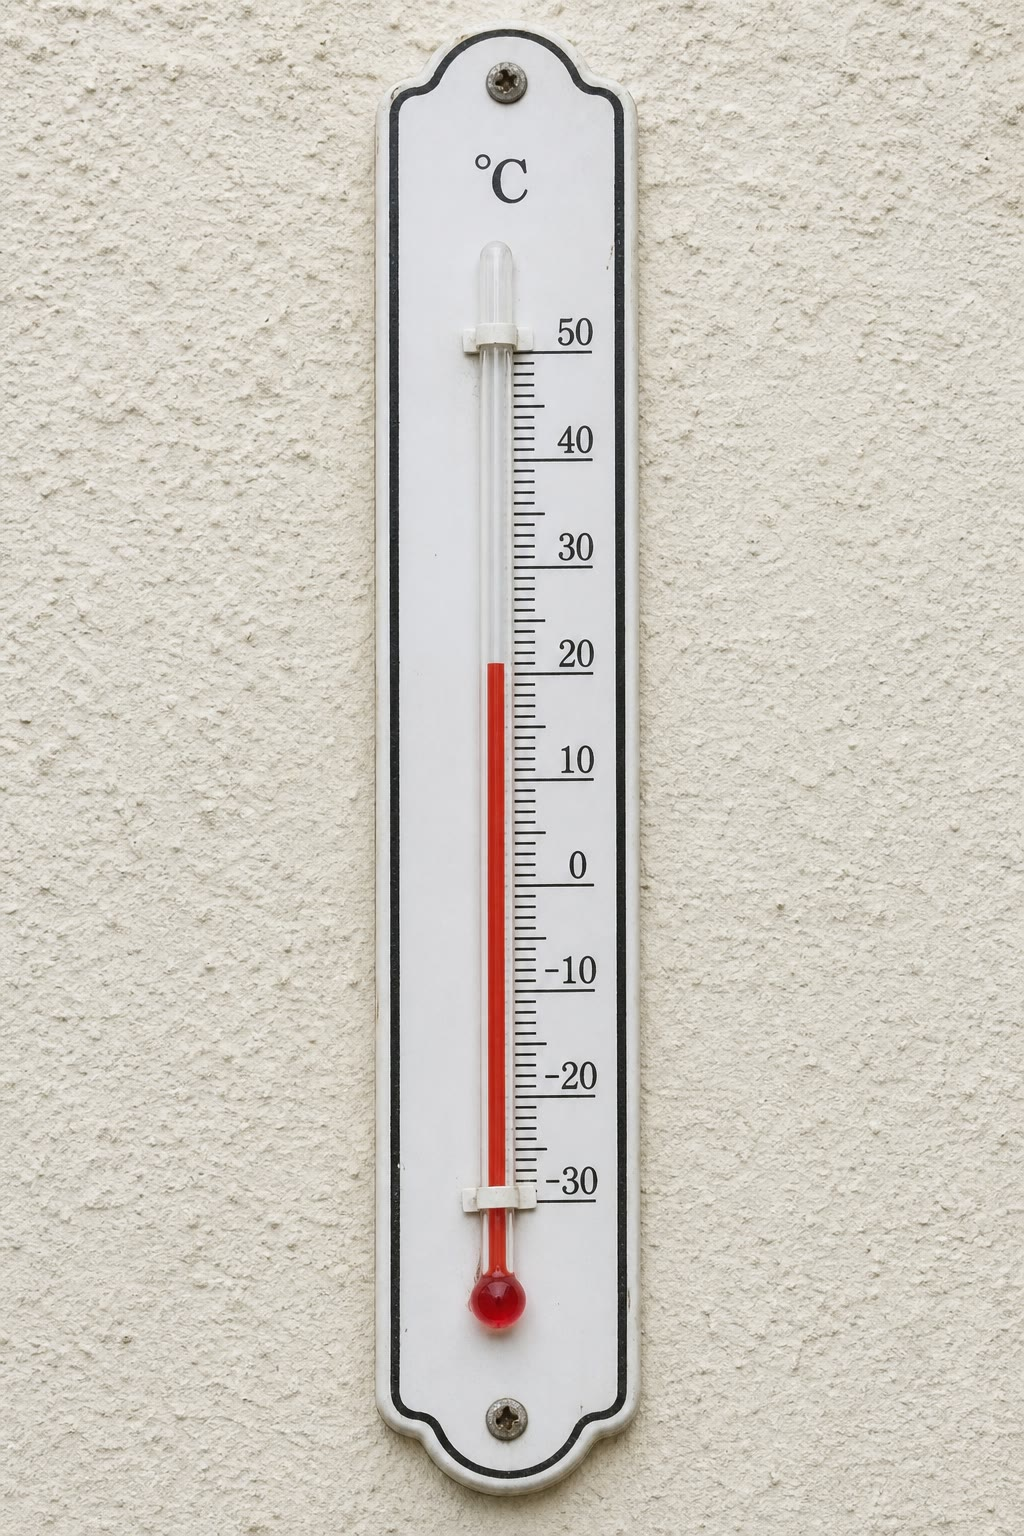
\includegraphics[width=0.3\linewidth]{images/book1/ai/g3-thermometer-outdoor.jpg}

{\small दीवार पर लगा असली \omterm{def:g3:temperature-thermometers:temperature}{तापमापी}: लाल स्तंभ मापनी पर चढ़ता है, और निशान पढ़ने वाले हर किसी को वही संख्या मिलती है।}
\end{omfigure}

\section{तापमापी पढ़ना}

\begin{method}[तापमापी पढ़ना]\label{met:g3:temperature-thermometers:read}
\begin{enumerate}
  \item \omterm{def:g3:temperature-thermometers:temperature}{तापमापी} को वहीं रखो जहाँ का \omterm{def:g3:temperature-thermometers:temperature}{ताप} जानना है --- पानी में, बाहर
        \omterm{def:g1:light-and-shadows:shadow}{छाया} में, या जीभ के नीचे;
  \item \emph{ठहरो} --- \omterm{def:g3:solids-liquids-gases:liquid}{द्रव} को चढ़ना या उतरना पूरा करने में समय
        लगता है; तब तक देखो जब तक वह रुक न जाए;
  \item अपनी आँख स्तंभ के सिरे के बराबर लाओ;
  \item स्तंभ जिस निशान तक पहुँचा है वहाँ की संख्या पढ़ो, और उसे
        उसके \omterm{def:g2:measuring-length:measure}{मात्रक} के साथ लिखो: \qty{18}{\celsius}।
\end{enumerate}
जल्दबाज़ी में या तिरछे कोण से पढ़ने पर संख्या ग़लत निकलती है --- जज
ईमानदार है, पर उससे सवाल ठीक ढंग से पूछना पड़ता है।
\end{method}

\begin{example}[काम आने वाले ताप]\label{ex:g3:temperature-thermometers:livedby}
कुछ संख्याएँ याद रखने लायक हैं: सुहावना कमरा लगभग
\qty{20}{\celsius} का होता है; तुम्हारा शरीर गरमी और जाड़े, दोनों में
ख़ुद को लगभग \qty{37}{\celsius} पर रखता है (उससे काफ़ी ऊपर जाना
बुख़ार है --- डॉक्टर का \omterm{def:g3:temperature-thermometers:temperature}{तापमापी} यह जानता है); फ़्रिज लगभग
\qty{4}{\celsius} पर रहता है; गरमी का तेज़ दिन \qty{30}{\celsius} तक
पहुँच जाता है; और नहाने का पानी \qty{35}{\celsius} के आस-पास सुहाता
है।
\end{example}

\begin{omfigure}
\begin{tikzpicture}[scale=0.85]
  \foreach \x/\h/\t/\name in {0/1.1/4/फ़्रिज,
      3.0/2.1/20/सुहावना कमरा, 6.0/3.0/37/तुम्हारा शरीर,
      9.0/2.6/30/गरमी का दिन} {
    \draw[thick] (\x,0) rectangle ++(0.42,3.6);
    \fill[omThm, opacity=0.7] (\x+0.08,0.05) rectangle ++(0.26,\h);
    \node[above, font=\footnotesize] at (\x+0.21,3.65)
      {$\t$\,\unit{\celsius}};
    \node[below, font=\small, align=center] at (\x+0.21,-0.2) {\name};
  }
\end{tikzpicture}

{\small जाने-पहचाने चार \omterm{def:g3:temperature-thermometers:temperature}{ताप}: स्तंभ जितना ऊँचा, चीज़ उतनी ही गरम।}
\end{omfigure}

\section{शून्य से नीचे}

\begin{example}[जाड़े की संख्याएँ]\label{ex:g3:temperature-thermometers:belowzero}
जमा देने वाली सुबह में स्तंभ $0$ के निशान से \emph{नीचे} उतर जाता
है। निशान वहाँ भी नीचे की ओर चलते रहते हैं, और हम उन्हें ``ऋण'' शब्द
के साथ पढ़ते हैं: शून्य से एक निशान नीचे यानी \emph{ऋण एक} डिग्री,
पाँच निशान नीचे यानी \emph{ऋण पाँच}, जिसे \qty{-5}{\celsius} लिखते
हैं। ऋण वाली संख्याएँ शून्य से भी ठंडी होती हैं, और वे जितनी नीचे
जाएँ पाला उतना ही कड़ा: $-10$ वाली सुबह $-2$ वाली सुबह से ज़्यादा
काटती है। जाड़े की हर शाम मौसम का हाल यही संख्याएँ बताता है।
\end{example}

\begin{remark}[शून्य का मतलब ``कुछ नहीं'' नहीं है]\label{rem:g3:temperature-thermometers:zero}
इस मापनी पर $0$ का मतलब ``\omterm{def:g3:temperature-thermometers:temperature}{ताप} ही नहीं'' नहीं है --- वह तो बस वह
निशान है जहाँ पानी \omterm{def:g2:ice-water-steam:meltfreeze}{जमता} है, सड़क के मील-पत्थर जैसा। मौसम उस
मील-पत्थर से गरम भी हो सकता है और ठंडा भी; \omterm{def:g3:temperature-thermometers:temperature}{तापमापी} सिर्फ़ यह बताता है
कि तुम किस ओर हो और कितने निशान दूर। (शून्य से नीचे की संख्याओं का
अपना पूरा गणित है --- तुम्हारा गणित का पाठ्यक्रम उसे किसी आगे वाले
वर्ष में ठीक से उठाएगा।)
\end{remark}

\section{अभ्यास}

\begin{exercise}[$\star$]\label{exo:g3:temperature-thermometers:1}
गरम-ठंडे का जज तुम्हारे हाथ से ज़्यादा निष्पक्ष \omterm{def:g3:temperature-thermometers:temperature}{तापमापी} क्यों है?
पिछले अध्यायों से एक ऐसा मौक़ा बताओ जब हाथ धोखा खा गए थे।
\end{exercise}

\begin{exercise}[$\star$]\label{exo:g3:temperature-thermometers:2}
पानी किस \omterm{def:g3:temperature-thermometers:temperature}{ताप} पर \omterm{def:g2:ice-water-steam:meltfreeze}{जमता} है? किस पर उबलता है? दोनों संख्याएँ किस \omterm{def:g2:measuring-length:measure}{मात्रक}
में हैं?
\end{exercise}

\begin{exercise}[$\star$]\label{exo:g3:temperature-thermometers:3}
\omterm{def:g3:temperature-thermometers:temperature}{तापमापी} को गरम करने पर पतली नली के \omterm{def:g3:solids-liquids-gases:liquid}{द्रव} का क्या होता है? और ठंडा
करने पर? इतना छोटा बदलाव इतने साफ़ ढंग से क्यों दिख जाता है?
\end{exercise}

\begin{exercise}[$\star$]\label{exo:g3:temperature-thermometers:4}
\cref{met:g3:temperature-thermometers:read} \omterm{def:g3:temperature-thermometers:temperature}{तापमापी} पढ़ते समय
जिन दो ग़लतियों से सावधान करती है, उन्हें गिनाओ।
\end{exercise}

\begin{exercise}[$\star$]\label{exo:g3:temperature-thermometers:5}
हर चीज़ को उसके संभावित \omterm{def:g3:temperature-thermometers:temperature}{ताप} से जोड़ो --- \qty{4}{\celsius},
\qty{20}{\celsius}, \qty{37}{\celsius}, \qty{100}{\celsius}: उबलता
पानी; \ आरामदेह बैठक; \ फ़्रिज के भीतर; \ तुम्हारा अपना शरीर।
\end{exercise}

\begin{exercise}[$\star$]\label{exo:g3:temperature-thermometers:6}
नहाने के पानी का \omterm{def:g3:temperature-thermometers:temperature}{तापमापी} \qty{35}{\celsius} बताता है; चूल्हे पर रखा
पतीला \qty{100}{\celsius}। कौन ज़्यादा गरम है, और क्या पतीला छूना
सुरक्षित है? पतीला नहाने के पानी से कितनी डिग्री ज़्यादा गरम है?
\end{exercise}

\begin{exercise}[$\star$]\label{exo:g3:temperature-thermometers:7}
जाड़े का एक \omterm{def:g3:temperature-thermometers:temperature}{तापमापी} स्तंभ को शून्य से $3$ निशान नीचे दिखाता है। इस
\omterm{def:g3:temperature-thermometers:temperature}{ताप} को हम कैसे कहते और लिखते हैं? यह \qty{-8}{\celsius} से ठंडा है
या गरम?
\end{exercise}

\begin{exercise}[$\star$]\label{exo:g3:temperature-thermometers:8}
कल बग़ीचे के \omterm{def:g3:temperature-thermometers:temperature}{तापमापी} ने नाश्ते के समय \qty{6}{\celsius} और दोपहर के
खाने के समय \qty{14}{\celsius} बताया था। सुबह कितनी डिग्री गरम हुई?
\end{exercise}

\begin{exercise}[$\star$]\label{exo:g3:temperature-thermometers:9}
रात भर में सड़क के गड्ढों का पानी बर्फ़ बन गया है। बिना किसी \omterm{def:g3:temperature-thermometers:temperature}{तापमापी}
के तुम रात के \omterm{def:g3:temperature-thermometers:temperature}{ताप} के बारे में क्या कह सकते हो? तुम कौन-सा मील-पत्थर
काम में ले रहे हो?
\end{exercise}

\begin{exercise}[$\star\star$]\label{exo:g3:temperature-thermometers:10}
बर्फ़ पर फिसलने के तुरंत बाद एम्मा दौड़कर गलियारे में आती है और
चिल्लाती है, ``यहाँ तो आग बरस रही है!'' गलियारे का \omterm{def:g3:temperature-thermometers:temperature}{तापमापी}
\qty{16}{\celsius} बताता है। क्या गलियारा गरम है? एम्मा को ऐसा लगता
क्यों है --- और घर वालों को किस जज पर भरोसा करना चाहिए?
\end{exercise}

\begin{exercise}[$\star\star$]\label{exo:g3:temperature-thermometers:11}
एक रसोइया जानना चाहती है कि खौलता सूप जितनी देर उबले उतना ही गरम
होता जाता है या नहीं। वह मापती है: एक मिनट उबलने के बाद
\qty{100}{\celsius}; दस मिनट बाद भी \qty{100}{\celsius}। \omterm{def:g3:temperature-thermometers:temperature}{तापमापी} उसे
उबलते पानी के बारे में --- और पानी के मील-पत्थरों के बारे में ---
क्या सिखाता है?
\end{exercise}
